%\emph{•}%%%%%%%%%%%%%%%%%%%%%%%%%%%%%%%%%%%%%%%%%
% Short Sectioned Assignment
% LaTeX Template
% Version 1.0 (5/5/12)
%
% This template has been downloaded from:
% http://www.LaTeXTemplates.com
%
% Original author:
% Frits Wenneker (http://www.howtotex.com)
%
% License:
% CC BY-NC-SA 3.0 (http://creativecommons.org/licenses/by-nc-sa/3.0/)
%
%%%%%%%%%%%%%%%%%%%%%%%%%%%%%%%%%%%%%%%%%
%----------------------------------------------------------------------------------------
%	PACKAGES AND OTHER DOCUMENT CONFIGURATIONS
%----------------------------------------------------------------------------------------
\documentclass[norsk]{article} % A4 paper and 11pt font size

\usepackage[T1]{fontenc} % Use 8-bit encoding that has 256 glyphs
\usepackage{fourier} % Use the Adobe Utopia font for the document - comment this line to return to the LaTeX default
\usepackage[english]{babel} % English language/hyphenation
\usepackage{amsmath,amsfonts,amsthm} % Math packages

% Added by Haavard %---------------------------------------------------------------------
\usepackage[utf8]{inputenc} % Norwegian letters
\usepackage{fullpage}
\usepackage{subcaption}
\usepackage[font={small, it}]{caption} % captions on figures and tables
\usepackage{graphicx}
\usepackage{color}
\usepackage{hyperref} % Use \autoref{ and \nameref{
\hypersetup{backref,
  colorlinks=true,
  breaklinks=true,
  %hidelinks, %uncomment to make links black
  linkcolor=blue,
  urlcolor=blue,
  citecolor=blue
}
\usepackage[all]{hypcap} % Makes hyperref jup to top of pictures and tables
% --------------------------------------------------------------------------------------

% Added by Jorgen, for source code listing %-------------------------------------------
\usepackage{wrapfig}

\usepackage{listings}
\usepackage{xcolor}
\newcommand{\textcolordummy}[2]{#2}

\definecolor{mygray}{rgb}{0.4,0.4,0.4}
%\definecolor{mycyan}{rgb}{0,0.8,0.6}
\definecolor{mygreen1}{rgb}{0.3,0.6,0.3}
\definecolor{mygreen2}{rgb}{0,0.4,0.1}
\definecolor{myorange}{rgb}{1.0,0.4,0}

\lstset{language=C++,
                basicstyle={\color{black}\footnotesize\ttfamily\let\textcolor\textcolordummy},
                %identifierstyle=\color{green},
                keywordstyle={\color{blue}\footnotesize\ttfamily\let\textcolor\textcolordummy},
                %keywordstyle={\color{blue}\footnotesize\ttfamily\let\textcolor\textcolordummy},
                directivestyle={\color{mygreen1}},
                emph={int,char,double,float,unsigned},
                emphstyle={\color{mygreen2}},
                %
                stringstyle={\color{myorange}\footnotesize\ttfamily\let\textcolor\textcolordummy},
                %stringstyle={\color{orange}\footnotesize\ttfamily\let\textcolor\textcolordummy},
                commentstyle={\color{mygray}\footnotesize\ttfamily\let\textcolor\textcolordummy},
                morecomment=[l][\color{magenta}]{\#}
                %
                showspaces=false,  
                showstringspaces=false, 
                showtabs=false,
                extendedchars=true,
                frame=single,  
}
\lstdefinestyle{FormattedNumber}{%
    literate={0}{{\textcolor{red}{0}}}{1}%
             {1}{{\textcolor{red}{1}}}{1}%
             {2}{{\textcolor{red}{2}}}{1}%
             {3}{{\textcolor{red}{3}}}{1}%
             {4}{{\textcolor{red}{4}}}{1}%
             {5}{{\textcolor{red}{5}}}{1}%
             {6}{{\textcolor{red}{6}}}{1}%
             {7}{{\textcolor{red}{7}}}{1}%
             {8}{{\textcolor{red}{8}}}{1}%
             {9}{{\textcolor{red}{9}}}{1}%
             {.0}{{\textcolor{red}{.0}}}{2}% Following is to ensure that only periods
             {.1}{{\textcolor{red}{.1}}}{2}% followed by a digit are changed.
             {.2}{{\textcolor{red}{.2}}}{2}%
             {.3}{{\textcolor{red}{.3}}}{2}%
             {.4}{{\textcolor{red}{.4}}}{2}%
             {.5}{{\textcolor{red}{.5}}}{2}%
             {.6}{{\textcolor{red}{.6}}}{2}%
             {.7}{{\textcolor{red}{.7}}}{2}%
             {.8}{{\textcolor{red}{.8}}}{2}%
             {.9}{{\textcolor{red}{.9}}}{2}%
             ,
   basicstyle=\footnotesize\ttfamily,%  Optional to use this
}

%---------------------------------------------------------------------

\usepackage{lipsum} % Used for inserting dummy 'Lorem ipsum' text into the template

\usepackage{sectsty} % Allows customizing section commands
\allsectionsfont{\centering \normalfont\scshape} % Make all sections centered, the default font and small caps

\usepackage{fancyhdr} % Custom headers and footers
\pagestyle{fancyplain} % Makes all pages in the document conform to the custom headers and footers
\fancyhead{} % No page header - if you want one, create it in the same way as the footers below
\fancyfoot[L]{} % Empty left footer
\fancyfoot[C]{} % Empty center footer
\fancyfoot[R]{\thepage} % Page numbering for right footer
\renewcommand{\headrulewidth}{0pt} % Remove header underlines
\renewcommand{\footrulewidth}{0pt} % Remove footer underlines
\setlength{\headheight}{13.6pt} % Customize the height of the header

\numberwithin{equation}{section} % Number equations within sections (i.e. 1.1, 1.2, 2.1, 2.2 instead of 1, 2, 3, 4)
\numberwithin{figure}{section} % Number figures within sections (i.e. 1.1, 1.2, 2.1, 2.2 instead of 1, 2, 3, 4)
\numberwithin{table}{section} % Number tables within sections (i.e. 1.1, 1.2, 2.1, 2.2 instead of 1, 2, 3, 4)

\setlength\parindent{0pt} % Removes all indentation from paragraphs - comment this line for an assignment with lots of text

%----------------------------------------------------------------------------------------
%	TITLE SECTION
%----------------------------------------------------------------------------------------

\newcommand{\horrule}[1]{\rule{\linewidth}{#1}} % Create horizontal rule command with 1 argument of height

%\title{	
%\normalfont \normalsize 
%\textsc{NTNU} \\ [25pt] % Your university, school and/or department name(s)
%\horrule{0.5pt} \\[0.4cm] % Thin top horizontal rule
%\huge C++  Notes \\ % The assignment title
%\horrule{2pt} \\[0.5cm] % Thick bottom horizontal rule
%}

%\author{Jørgen Vågan} % Your name

%\date{\normalsize\today} % Today's date or a custom date

\begin{document} %---------------------------------------

%\maketitle % Print the title

\section{Spørsmål Runde 1 }
%Jeg har funnet et program kalt \textbf{Engauge Digitizer} til å lese av grafene. Sliter litt med 
%at den ikke identifiserer alle kurvene og sliter med overlappende biter.
%\newline
%\begin{wrapfigure}{r}{0.6\textwidth} %Requires the package wrapfigure
  %\begin{center}
    %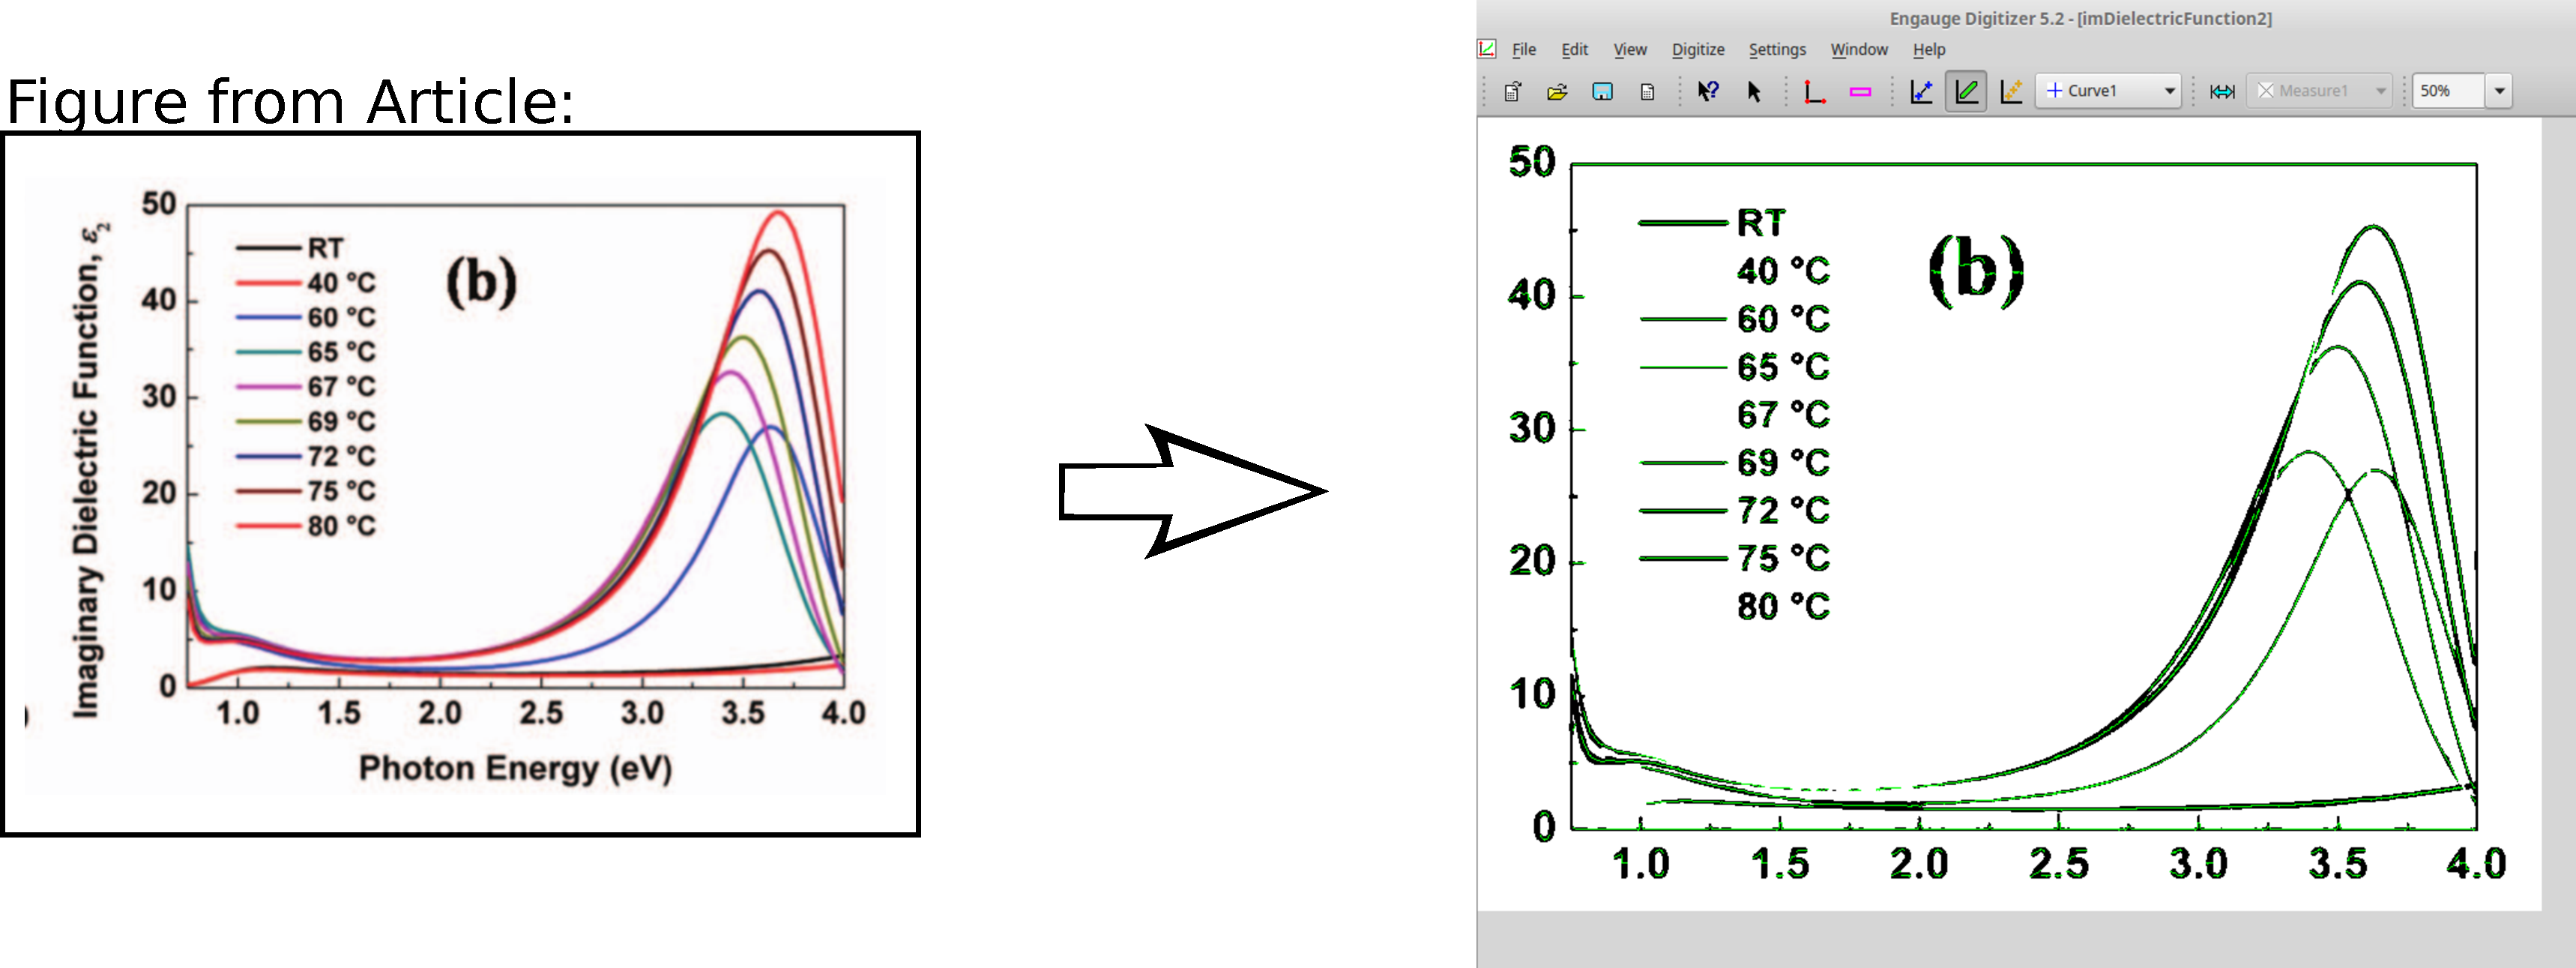
\includegraphics[width=0.58\textwidth]{engaugeExample.pdf}
  %\end{center}
%\end{wrapfigure}
Jeg prøver å forstå mer detaljert hvordan jeg skal få lest inn dataen til GranFilm programmet.
Formatet til ''.nk''-filene i \texttt{GranFilm/Sopra/DataBase} ser slik ut (her mgo.nk):
\begin{lstlisting}[style=FormattedNumber,frame=none]
   1		0.65			10		400    
        1.70969699     0.00000011
        1.71065583     0.00000011
        1.71239613     0.00000011
\end{lstlisting}
og ser ut til å ha reell og imaginær refraksjonsindeks forholdsvis på kolonne 1 og 2. I tillegg virker det
som om rad èn består av de 4 verdiene: 
\begin{itemize}
   \item unit (om refraksjonsindeksen er funksjon av energi (eV) 
eller bølgelengde); 
\item x startverdi (energi/bølgelengde); 
\item x sluttverdi
\item antall datapunkter.
\end{itemize}
Basert på dette, i tillegg til modulen fra source-koden til GranFilm gitt nedenfor, virker det
som om reell og imaginær verdi er gitt for samme x-verdi (energi/bølgelengde), der x-verdiene 
har konstant steglengde. (For eksempel: for mgo.nk filen ville vi hatt $d\!x = \frac{10-0.65}{400-1}$).
\\
\\
Jeg har funnet et program som lar meg hente ut dataen fra grafer i artikklene. 
Prolemet er at dataen for reell og imaginær refraksjonsindeks 
er for forskjellige x-verdier, der x-verdiene ikke har
konstant steglengde.\\
\\
\textbf{Spørsmålene er derfor:} 
\begin{enumerate}
   \item Er det riktig det jeg har forstått ovenfor? 
   \item Trenger jeg skrive om inputfilene (filene med thermochrom-dataen) 
      slik at reell og imaginær verdi (forholdsvis $n$,$k$)
      svarer til samme x-verdi, der x-verdiene ligger med avstand $d\!x$ i fra hverandre?\\
      (Jeg tenkte å kanskje skrive en funksjon som tar inn to filer, colonner og ''unit''-verdi, 
      leser inn $n$ og $k$ dataen fra filene, intrapolerer for felles, nye x-verdier og skriver til 
      en ny fil.)
   \item Videre: noen grafer er gitt ved permittivitet $\varepsilon$, istedenfor refraksjonsindex \textbf{n}.
      Da er det vel bare å regne om ved bruk av imaginær permittivitet? Jeg fant noen formlet og lurte på 
      om dette er riktig: fant at 
      \begin{align*}
         \boldsymbol{\varepsilon} =
            \frac{c^2 \varepsilon_0}{\omega^2 \frac{\mu}{mu_0}} \Bigg( k^2 - \frac{\alpha ^2}{4}\Bigg)  
            + i\Bigg( \frac{c^2 \varepsilon_0}{\omega^2 \frac{\mu}{\mu_0}} k \alpha \Bigg)
      \end{align*}
      ($k$ er hær bølgetallet), hvor 
      \begin{align*}
         &\boldsymbol{n} = k - i\frac{\alpha}{2}, & \boldsymbol{n} = \frac{c}{\omega} \boldsymbol{k}^*.
      \end{align*}
      Bruker at $\mu = \mu_0$ og får
      \begin{align*}
         &\text{Re}(n) = \frac{\text{Im}(\varepsilon)}{2 \varepsilon_0} \\
         &\text{Im}(n) = \sqrt{\frac{\text{Re}(\varepsilon)}{\varepsilon_0} - 
         \Bigg( \frac{\text{Im}(\varepsilon)}{2 \varepsilon_0} \Bigg) ^2}.
      \end{align*}
\end{enumerate}

Til slutt vil jeg bare si at framgangen går sakte, og begynner å bli litt stresset mtp tiden. Lurte
på hvor mye du hadde forestilt deg at jeg burde få til? Foreløpig, har jeg klart å lese ut 
VO$_2$-dataen fra de fire artiklene du sendte meg. Dataene trenger trolig mer arbeid før de mates inn
i GranFilm som beskrevet ovenfor. Der ligger VO$_2$ data for 10-12 forskjellige temperaturer.


%I kildekoden til \texttt{GranFilm} fant jeg \texttt{dielectric\_function\_module.f90}:
%\begin{lstlisting}[style=FormattedNumber,frame=none, language=FORTRAN]
    %Read(unit=ifile,fmt=*) unit,x1,x2,lines
    %dx = (x2 - x1)/(lines-1)

    %Allocate( x(lines), y(lines) )
    %Select Case (unit)
    %Case(1)
       %! Unit = Electron Volt (eV)
       %Do i=1,lines 
          %Read(unit=ifile,fmt=*) tmp(1), tmp(2)
          %x(i) = x1 + (i-1)*dx
          %y(i) = tmp(1)+imu*tmp(2)
       %Enddo
    %Case(2)
       %! Unit = WaveLength (microm)
       %Do i=lines,1,-1 
          %Read(unit=ifile,fmt=*) tmp(1), tmp(2)
          %x(i) = x1 + (lines-i)*dx
          %y(i) = tmp(1)+imu*tmp(2)
       %Enddo
       %x(:) = 1.243\_wp/x(:) ! Conversion microm-->eV
    %End Select

    %Close(unit=ifile)
%\end{lstlisting}
%først leses første linje av \texttt{'.nk'}-filen:
%som gir \texttt{unit} (som er hva?), start energi/bølgelengde, slutt energi/bølgelengde og til slutt 
%antall datapunkter. Når du nå regner ut \texttt{x} og \texttt{y} virker det som om du antar at
%n,k-verdiene er gitt from samme energi(eV) eller bølgelengde. I tillegg virker det som at datapunktene
%må være separert med konstant steglengde $dx$. Men, i mine avleste data
%er ikke dette tilfellet: dataen er gitt for ulike verdier og steglengden varierer: 
%\begin{lstlisting}[style=FormattedNumber,frame=none]
   %//#! Fra fil reIndexOfRefractionVO2.csv,
   %x,n06,n13
   %3.40909e-07,1.96538,1.01971
   %3.45455e-07,2.12453,1.15231
   %3.61364e-07,2.68154,1.61639
   %.           .       .
   %.           .       .
%\end{lstlisting}
%\begin{lstlisting}[style=FormattedNumber,frame=none]
   %//#! Fra fil imIndexOfRefractionVO2.csv
   %x,k06,k13
   %3.41541e-07,1.44393,0.928804
   %3.42121e-07,1.43807,0.933948
   %3.51121e-07,1.34701,1.01382
   %.           .       .
   %.           .       .
%\end{lstlisting}
%Må jeg passe på at input-data-filen er slik som jeg har tolket ovenfor, altså:
%to kolonner (første med reel refraksjonsindex og andre med imaginer refraksjonsindex)
%der verdiene i en gitt rad er gitt for samme x-verdi (energi/bølgelengde)?\\
%\\
%Hele koden for funksjonen er hær:
I kildekoden til \texttt{GranFilm} \: fant jeg modulen \: \texttt{dielectric\_function\_module.f90}.
Forstår det slik at 
\begin{lstlisting}[style=FormattedNumber, language=FORTRAN, frame=none]
    Function Locate(xx,x)
\end{lstlisting}
finner indeksen i xx til elementet som ligger nærmest verdien x? Tenkte å kunne bruke
funksjonen eller skrive den om, og bruke den i intrapolering om jeg må skrive om input-filene.
\begin{lstlisting}[style=FormattedNumber, language=FORTRAN]
  !------------------------------------------------------------!
  Subroutine Get_Dielectric_Function(energy,epsilon,material,path)
  !Subroutine dielectric_constants(energy,epsilon,material,path)
  !------------------------------------------------------------!
    Use SFL_Logical_Units,       only : SFL_Get_Free_Unit
    Use Error_Module,            only : Error_Failure
    Implicit None
    Real(wp)                          :: energy(:)
    complex(wp )                      :: Epsilon(:)
    Character(len=*)                  :: material
    Character(len=*)                  :: path
    ! --- Local
    Character(len=*), parameter       :: routine = "Get_Dielectric_Function"
    !complex(wp ),Parameter            :: im=(0._wp,1._wp)
    Character(len=250)                :: filename, str
    Logical                           :: exi
    integer                           :: lines,start,i, ifile
    Real(wp),     Allocatable         :: x(:)
    complex(wp ), Allocatable         :: y(:)
    Real(wp)                          :: tmp(2),x1,x2,dx
    integer                           :: unit, istat
    complex(wp )                      :: slope
    

    ! Opens the relevant data file for the given material
    ! Notice that the data-files contains the values for the 
    ! index of refraction, n,k extacted from the data base of
    ! SOPRA.
    ! Therefore "epsilon = epsilon**2" at the bottom of this routine    
    filename = Trim(Adjustl(path))//'/'//Trim(Adjustl(material))//'.nk'
    Inquire(file=Trim(Adjustl(filename)),exist = exi)
    If( .NOT. exi ) Then
       write(str,*) trim(adjustl(filename))
       str = "File = " // trim(adjustl(str)) // " non existing" 
       Call Error_Failure(routine, trim(adjustl(str)) )
    Endif
    call SFL_Get_Free_Unit( ifile )
    Open(unit=ifile,file=filename,status='old')
    Read(unit=ifile,fmt=*) unit,x1,x2,lines
    dx = (x2 - x1)/(lines-1)

    Allocate( x(lines), y(lines) )
    Select Case (unit)
    Case(1)
       ! Unit = Electron Volt (eV)
       Do i=1,lines 
          Read(unit=ifile,fmt=*) tmp(1), tmp(2)
          x(i) = x1 + (i-1)*dx
          y(i) = tmp(1)+imu*tmp(2)
       Enddo
    Case(2)
       ! Unit = WaveLength (microm)
       Do i=lines,1,-1 
          Read(unit=ifile,fmt=*) tmp(1), tmp(2)
          x(i) = x1 + (lines-i)*dx
          y(i) = tmp(1)+imu*tmp(2)
       Enddo
       x(:) = 1.243_wp/x(:) ! Conversion microm-->eV
    End Select

    Close(unit=ifile)

    ! --- Do the interpolation
    Do i=1,Size(energy,1)
       start=locate(x(:),energy(i))
       If((start==0).Or.(start==lines)) Then
          write(str,"('Energy not in range : ',f5.2,' for i=',i3)") energy(i),i
          call Error_Failure( routine, trim(adjustl(str)))
       Endif
       ! Linear interpolation
       slope = (y(start+1)-y(start))/(x(start+1)-x(start))
       Epsilon(i) = y(start) + slope*(energy(i)-x(start))
       !            Write(unit=67,*) energy(i),Real(epsilon(i)),Aimag(epsilon(i))
    Enddo
    
    ! --- Calculates the dielectric constant (from the refraction index)
    epsilon = epsilon**2
    Deallocate(x,y,stat=istat)

  contains
    
    Function Locate(xx,x)
      Implicit None
      Real(wp), Dimension(:), Intent(In)  :: xx
      Real(wp), Intent(In)                :: x
      Integer                             :: locate
      Integer                             :: n,jl,jm,ju
      Logical                             :: ascnd
      
      n=Size(xx)
      ascnd = (xx(n) >= xx(1))
      jl=0
      ju=n+1
      Do
         If(ju-jl <= 1) exit
         jm=(ju+jl)/2
         If(ascnd .eqv. (x >= xx(jm))) Then
            jl=jm
         Else
            ju=jm
         Endif
      Enddo
      If(x == xx(1)) Then
         locate=1
      Else If(x == xx(n)) Then
         locate=n-1
      Else
         locate=jl
      Endif
      
    End Function Locate
    

  End Subroutine Get_Dielectric_Function
  !-------------------------------------!
\end{lstlisting}



%\section{Theory}
To understand the theoretical background behind GranFilm and scattering on diffuse surfaces, it is 
convenient to start with the simple case of scattering on a flat interface of two different half-infinite
media, see Figure !!FIGUREREF HERE!!.

The electric permittivity $\varepsilon$ and magnetic permeability $\mu$ of the media are given with subscript $1$ for the above media, and $2$ for the media below. 
Using Maxwell's equations
%
\begin{subequations}
\label{ME}
\begin{align}
   \nabla \cdot \boldsymbol{D} &= \rho \!_f           &\nabla\times\boldsymbol{E} &= - \frac{\partial \boldsymbol{B}}{\partial t} \label{ME1}\\
   \nabla \cdot \boldsymbol{B} &= 0                &\nabla \times \boldsymbol{H}&= \boldsymbol{J}\!_f + \frac{\partial \boldsymbol{D}}{\partial t}, \label{ME2}
\end{align}
\end{subequations}
%
where the electric fields, $\boldsymbol{E}$ and $\boldsymbol{D}$, and magnetic fields $\boldsymbol{B}$ and $\boldsymbol{H}$ are related through
\begin{align}
   &\boldsymbol{D} = \varepsilon \boldsymbol{E},         &\boldsymbol{H} = \frac{1}{\mu} \boldsymbol{B}
\end{align}
(assuming linear media), the fields above $\boldsymbol{E}^+(\boldsymbol{r})$ and below $\boldsymbol{E}^-(\boldsymbol{r})$ the interface can be calculated for a incident place wave 
(same goes for $\boldsymbol{B}$, $\boldsymbol{D}$ and $\boldsymbol{H}$).
So far, the boundary between the two half-infinite media has been considered to be a sharp, flat discontinuity in $\varepsilon(z)$ and $\mu (z)$. 
As soon as the surface roughness, thickness and/or impurities are taken into acount, the complexity of the problem increases.


\textbf{From ''GranFilm-Software-Article''}: \\
Information on the dieletric behavior of surfaes can often be obtained by measuring the Fresnel coefficients,
such as reflection, transmission and absorption. \\
?p.2?: for a layer with thickness negligible compared to wavelength, we introduce surface susceptibilities 
which interconnect the  fresnel coeff. and characterise the optical response of the surface. ?? DID I UNDERSTAND THIS CORRECTLY? ?? \\
Since all the Fresnel coeff. can be expressed in terms of these surface susceptibilities, the main task consist of calculating these coefficients for the appropriate geometry. \\
\textbf{Goal of GranFilm:} to calculate ?surface-susceptibility-/fresnel-coefficients? and the associated measurableFresnel quantities for various surface layer geometries. 
\begin{itemize}
\item GranFilm is free open-source software
\end{itemize}
\subsection{Mie resonances/ plasmon absorption modes}
\textbf{From ''GranFilm-Software-Article''}: \\
when small metallic particles, the resonances can be absorbed by visible light and strongly affect the fresnel 
coefficients depending on the particle morphology.
%
\subsection{Quasistatic Approximation}
%
\subsection{Electromagnetic excess fields }
%
\textbf{From ''GranFilm-Software-Article''}: \\
(Bedeaux and Vlieger) \\
Difference between the bulk extrapolated fields and the real fields. The BC at the dividing surface
(which drive all fresnel coeff.) are given in terms of the integrated excess fields perpendicular to
the surface. \\
Bedeaux and Vlieger $\rightarrow$ formalism of excess quantities (does not require exact knowledge of the near suface EM-field behaviour). \\
Excess fields are defined as the differene between the real fields and the bulk fields extrapolated to the surface. E.g. for the electric field $E(r)$ the excess quantity is defined as
\begin{align}
   E_{ex} (r) = E(r) - E^-(r) \theta(-z) - E^+(r)\theta(z),
\end{align}
where $\theta(z)$ is the Heaviside function and the superscript $\pm$ are used to indicate the region above (+) and below (-) the dividing interface at $z = 0$. 
The excess field is only significant close to the surface, since $E(r, \omega) \rightarrow \rightarrow E^{\pm}(r,\omega)$  for $z \rightarrow \pm \infty$. \\
\textit{QUESTION: \@ Is the $E^{\pm}$ field solved for a infinite homogeneous medium of type (+) and (-) respectively  OR the field in simple two media interface scattering?} \\
\textbf{From Leif Amund Lies Msc Thesis}: \\
Since the excess fields will only be significant close to the surface, they may be thought of as perturbations to the simple case of flat interface. 
\textit{OWN INTERPRETATION: \@ This meas that the bulk fields are the fields created from scattering in the interface between two half-infinite media.} \\
Instead of tediously using the quasi-static-"no source"-BC, the excess fields defined as for the electric field above are inserted into the full Maxwell equations to derive new non-sharp boundary conditions.
The result reads
%
\textbf{From Leif Amund Lies Msc Thesis AND GranFilm-Article}: \\
%
\begin{subequations}
   \label{exFieldBC} % Excess Field Boundary Conditions
\begin{align}
   \big[ \boldsymbol{E}^+_{\parallel} (\boldsymbol{r}) - \boldsymbol{E}^-_{\parallel} (\boldsymbol{r}) \big] \bigg\rvert _{z = 0} 
       &= i \omega \hat{z} \times \! \boldsymbol{M}^s_{\parallel}(\boldsymbol{r}_{\parallel}) \:-\: \nabla\!_{\parallel} P^s_{z}(\boldsymbol{r}_{\parallel}) 
       \label{exFieldBC1} \\ 
   \big[ D^+_{z} (\boldsymbol{r}) - D^-_{z} (\boldsymbol{r}) \big] \bigg\rvert _{z = 0} 
      &= - \nabla\!_{\parallel} \boldsymbol{P}^s_{\parallel}(\boldsymbol{r}_{\parallel}) 
      \label{exFieldBC2} \\ 
   \big[ \boldsymbol{H}^+_{\parallel} (\boldsymbol{r}) - \boldsymbol{H}^-_{\parallel} (\boldsymbol{r}) \big] \bigg\rvert _{z = 0} 
      &= i \omega \hat{z} \times \! \boldsymbol{P}^s_{\parallel}(\boldsymbol{r}_{\parallel}) \:-\: \nabla\!_{\parallel} M^s_{z}(\boldsymbol{r}_{\parallel})  
      \label{exFieldBC3} \\ 
   \big[ B^+_{z} (\boldsymbol{r}) - B^-_{z} (\boldsymbol{r}) \big] \bigg\rvert _{z = 0} 
      &= - \nabla\!_{\parallel} \boldsymbol{M}^s_{\parallel}(\boldsymbol{r}_{\parallel}), 
      \label{exFieldBC4}  
\end{align}
\end{subequations}
%
which is derived in Vlieger and Bedaux's \textit{Optical Properties of Surfaces} (p.21). Here the quantities with superscript $s$ are the so-called excess polarization and magnetization densities
\begin{subequations}
\label{surfQuant} %Surface Quantities
\begin{align}
   \boldsymbol{P}^s(\boldsymbol{r}\!_{\parallel}) &= \big( \boldsymbol{D}^s_{\parallel}(\boldsymbol{r}\!_{\parallel}), \:\: - \varepsilon_0 E^s_{z}(\boldsymbol{r}\!_{\parallel}) \big) \label{surfQuant1}\\
   \boldsymbol{M}^s(\boldsymbol{r}\!_{\parallel}) &= \big( \boldsymbol{B}^s_{\parallel}(\boldsymbol{r}\!_{\parallel}), \:\: - \mu_0 H^s_{z}(\boldsymbol{r}\!_{\parallel}) \big) , \label{surfQuant2}
\end{align}
\end{subequations}
and the quantities on the right hand side are the excess fields integrated along the z-axis,
\begin{subequations}
\label{intExQuant} % integrated excess quantities
\begin{align}
   \boldsymbol{D}^s_{\parallel}(\boldsymbol{r}) &= \!\!\!\!\!\!\!\!\! \int\limits ^{\:\:\:\:\:\:\:\:\:\:+\infty}_{\!\!\!\!\!\!\!\!\!\!\!\!\!\!\!-\infty} \!\!\!\!\!\!\!\!\! d\!z\: \boldsymbol{D}\!_{ex,\parallel}(\boldsymbol{r}),
   &E^s_{z}(\boldsymbol{r}) = \!\!\!\!\!\!\!\!\! \int\limits ^{\:\:\:\:\:\:\:\:\:\:+\infty}_{\!\!\!\!\!\!\!\!\!\!\!\!\!\!\!-\infty} \!\!\!\!\!\!\!\!\! d\!z\: E\!_{ex,z}(\boldsymbol{r}) \label{intExQuant1}\\
   \boldsymbol{B}^s_{\parallel}(\boldsymbol{r}) &= \!\!\!\!\!\!\!\!\! \int\limits ^{\:\:\:\:\:\:\:\:\:\:+\infty}_{\!\!\!\!\!\!\!\!\!\!\!\!\!\!\!-\infty} \!\!\!\!\!\!\!\!\! d\!z\: \boldsymbol{B}\!_{ex,\parallel}(\boldsymbol{r}),
   &H^s_{z}(\boldsymbol{r}) = \!\!\!\!\!\!\!\!\! \int\limits ^{\:\:\:\:\:\:\:\:\:\:+\infty}_{\!\!\!\!\!\!\!\!\!\!\!\!\!\!\!-\infty} \!\!\!\!\!\!\!\!\! d\!z\: H\!_{ex,z}(\boldsymbol{r}). \label{intExQuant2}
\end{align}
\end{subequations}
\textit{OWN INTERPRETATION: These integrated excess quantities are equivalent of representing the the excess fields in a single Dirac term $\delta (z)$ located at the surface ($z = 0$), e.g. such that the electric field can be 
written as}
%
\begin{align}
   E(r) =  E^-(r) \theta(-z) + E^s(r)\delta (z) +  E^+(r)\theta(z).
\end{align}
%
\textit{OWN INTERPRETATION: Demanding that this fullfuls Maxwell's Equations, one obtains the Equations in \eqref{exFieldBC} }.
\textit{OWN INTERPRETATION: The simplest way to link the Surface polarization and magnetization density to the extrapolated bulk fields(?Sigma indexed fields?)involves a
symmetric constitutive tensor $\xi^s_e(\omega)$ (ref B,V-OPoS).}
\begin{align}
   \boldsymbol{P}^s(\boldsymbol{r}\!_{\parallel}) = \xi ^s_e \: \big[ \boldsymbol{E}_{\parallel, \Sigma}(\boldsymbol{r}\!_{\parallel}), \:\: - D\!_{z, \Sigma}(\boldsymbol{r}\!_{\parallel}) \big]
\end{align}
\textit{OWN INTERPRETATION: The above relation is restricted to non-magnetic materials, i.e. that $\boldsymbol{M}^s(\boldsymbol{r}\!_{\parallel}) = 0$.   The $\Sigma$ index denotes the arithmetic mean of the upper and lower
bulk fields, e.g. $ \boldsymbol{E}_{\parallel, \Sigma} = \big\{ \boldsymbol{E}^+_{\parallel} \!( \boldsymbol{r}\!_{\parallel} ) +  \boldsymbol{E}^-_{\parallel} \! (\boldsymbol{r}\!_{\parallel}) \big\} \big/2 $.
If the interface are z = 0 is isotropic and symmetric, the interfacial tensor $\xi ^s_e$ is diagonal}:
\begin{align}
\xi ^s_e = 
\begin{bmatrix}
   \gamma   &   0       &  0      \\
   0        &   \gamma  &  0      \\
   0        &   0       &  \beta 
\end{bmatrix}
.
\end{align}
Here the coefficients $\gamma$ and $\beta$ are called the (first-order) surface susceptibilities (or here, constitutive coefficients). The constitutive coefficients of second order, $\delta$ and $\tau$ describe
a non-local dependence (??SPATIAL VARIATIONS IN THE EXCESS QUANTITIES??) \\
\textbf{Fresnel Coefficients} \\
...need to write some more here...
\begin{subequations}
   \label{fresCoeffS}
\begin{align}
   r_s(\omega) &= \frac{n\!_{_-} \cos \theta_i - n\!_{_+} \cos \theta_t + i(\omega/c) \gamma}{n\!_{_-} \cos \theta_i + n\!_{_+} \cos \theta_t - i(\omega/c) \gamma} \label{fresCoeffS1} \\
   t_s(\omega) &= \frac{2 n\!_{_-} \cos \theta_i}{n\!_{_-} \cos \theta_i + n\!_{_+} \cos \theta_t - i(\omega/c) \gamma} \label{fresCoeffS2}
\end{align}
\end{subequations}
%
\begin{subequations}
\label{fresCoeffP}
\begin{align}
   r_p(\omega) &= \frac{\kappa\!_{_-}(\omega) -i(\omega / c) \gamma \cos \theta_i \cos \theta_t + i(\omega/c)n\!_{_-} n\!_{_+} \varepsilon\!_{_-}\beta\sin^2 \theta_i }
   {\kappa\!_{_+}(\omega) -i(\omega / c) \gamma \cos \theta_i \cos \theta_t - i(\omega/c) n\!_{_-} n\!_{_+} \varepsilon\!_{_-} \beta \sin^2 \theta_i }, \label{fresCoeffS1}\\
   t_p(\omega) &= \frac{2n\!_{_-} \cos \theta_i \big[ 1 + (\omega/2c)^2 \varepsilon\!_{_-} \gamma \beta \sin ^2 \theta_i \big]}
   {\kappa\!_{_+}(\omega) -i(\omega / c) \gamma \cos \theta_i \cos \theta_t - i(\omega/c) n\!_{_-} n\!_{_+} \varepsilon\!_{_-} \beta \sin^2 \theta_i }, \label{fresCoeffS2}\\
   \kappa\!_{\pm} &= \big[ n\!_{_+} \cos \theta _i \pm n\!_{_-} \cos \theta_t  \big]\Bigg[ 1 - \frac{\omega^2}{4c^2} \varepsilon\!_{_-} \gamma \beta \sin ^2 \theta_i \Bigg]. \label{fresCoeffS3}
\end{align}
\end{subequations}
%
%\begin{subequations}
%\begin{align}
   %r_p(\omega) &= \frac{\kappa _-(\omega) -i(\omega / c) \gamma \cos \theta_i \cos \theta_t + i(\omega/c)n_-n_+\varepsilon_-\beta\sin^2 \theta_i }
               %{\kappa _+(\omega) -i(\omega / c) \gamma \cos \theta_i \cos \theta_t - i(\omega/c)n_-n_+\varepsilon_-\beta\sin^2 \theta_i } \\
   %t_p(\omega) &= \frac{2n_- \cos \theta_i \big[ 1 + (\omega/2c)^2 \varepsilon_- \gamma \beta \sin ^2 \theta_i \big]}
               %{\kappa _+(\omega) -i(\omega / c) \gamma \cos \theta_i \cos \theta_t - i(\omega/c)n_-n_+\varepsilon_-\beta\sin^2 \theta_i } \\
   %\kappa_{\pm} &= \big[ n_+ \cos \theta _i \pm n_- \cos \theta_t  \big]\Bigg[ 1 - \frac{\omega^2}{4c^2} \varepsilon_- \gamma \beta \sin ^2 \theta_i \Bigg]
%\end{align}
%\end{subequations}
From Eq. \eqref{fresCoeff1}-Eq.\eqref{fresCoeff3} we can observe that $p$-polarized excite the surface in both parallel and perpendicular direction, relative to the surface. 






\subsection{.}


\textbf{D'Alembert Operator $\square$}
\begin{align*}
  \square  &= \partial ^{\mu} \partial _{\mu}
   \\
           &= \frac{1}{c^2} \frac{\partial ^2}{\partial t^2} 
               - \frac{\partial ^2}{\partial x^2} 
               - \frac{\partial ^2}{\partial y^2} 
               - \frac{\partial ^2}{\partial z^2} 
   \\
           &= \frac{1}{c^2} \frac{\partial ^2}{\partial t^2} - \nabla ^2
\end{align*}

\textbf{Lorentz Gauge:} \\
For Lorentz invariance, convenient to choose the Lorenz gauge:
\begin{align*}
   \square \vec{A} = \Bigg[ \frac{1}{c^2} \frac{\partial ^2}{\partial t^2} - \nabla ^2 \Bigg] \vec{A} = \mu_0 \vec{J}
\end{align*}
\begin{align*}
   \square \phi = \Bigg[ \frac{1}{c^2} \frac{\partial ^2}{\partial t^2} - \nabla ^2 \Bigg] \phi = \frac{\rho}{\epsilon _0}
\end{align*}






%
\end{document}
